\section{Methodology}
\subsection{Direct Simulation Monte Carlo method}
The Direct Simulation Monte Carlo method  was initially introduced by Graeme A. Bird in the 1960s, and has become with time the de facto standard for rarefied flow simulations. When it was first developed, this method represented a radical departure from the traditional approaches employing a mathematical description of the flow, to such an extent that many questioned the validity of its results. It was eventually proven though, that, for time step and cell size tending to zero, the DSMC method converges to a solution of the Boltzmann equation \cite{bird}.

This method models the gas as a large collection of simulated particles, each representing an even wider set of real molecules. These molecules are propagated through the simulation domain, where they collide in a stochastic manner. \cite{themontecarlo}.

As the name in itself implies, this method is statistical at heart. Its results are in fact based on averaging the microscopic quantities of each of the molecules over a high number of time steps and over the grid cell size, in order to obtain global aerodynamic quantities. \cite{bird, themontecarlo}. This process will be discussed more in depth in \autoref{subsection:sampling}

\subsubsection{Particle description}
As mentioned previously, DSMC employs a particle description of the flow. The number of simulated particles is usually significantly lower than the real number of particles in the problem. This is due to the immense computational expense that simulating all of the particles in the real domain would require \cite{natodsmc}. To provide some perspective, it is useful to consider one of the most rarefied simulations conducted as part of this thesis. In this scenario, with a Knudsen number of 10 and a density of \SI{2e-7}{\kg\per\meter^3} (a mere 0.00001\% of the air density at sea level), more than \SI{3.6e18}{} molecules per cubic meter would have been required if a one-to-one correlation between the real and simulated molecules were to be maintained. The ratio between real and simulated molecules is expressed by $f_{num}$.

At the beginning of each simulation, a reference set of simulation particles is created. The microscopic properties (position and velocity) of each of the molecules in this set are chosen such that the bulk velocity and the global temperature of the flow correspond to the ones specified by the user, and that the number of simulated particles in the domain is equal to $\frac{n_{real}}{f_{num}}$. The velocity of the particles is usually selected through the Maxwell-Boltzmann distribution \cite{natodsmc}.

The simulated particles are not identical to the real particles: to correctly simulate the behaviour of the system the radius of each simulated particle must be proportional to the number of real particles that it represents, and is thus calculated such that \autoref{eq:radius} is valid. This approach also ensures the correct number of collisions in the flow \cite{dsmcnotes}.
\begin{equation}
    n_{real}\, \sigma_{real} = n_{sim}\, \sigma_{sim}
    \label{eq:radius}
\end{equation}
No indication of how the mass of each of the simulated particles is determined has been found in literature. However, based on how the SPARTA DSMC code calculates surface quantities, it is the author's understanding that the mass of the simulated particles is equal to the mass of the real particles.

\subsubsection{Mesh}
The DSMC method discretises the domain into a collection of mesh elements. This might seem counter intuitive, as the method operates on a particle-based description of the flow, which does not require the solution of any partial differential equation.

The mesh discretisation serves two main purposes: 

\begin{itemize}
    \item It allows to reduce the computational expense: employing pure Newtonian mechanics for all the molecules within the simulation domain would be too computationally expensive \cite{themontecarlo}. Thus DSMC only computes collision of randomly selected molecules within the same cell, disregarding collisions between molecules belonging to different cells, significantly cutting the computational burden. This topic will be discussed in more detail in \autoref{subsection:collision}
    \item It allows the calculation of global quantities such as temperature, bulk flow velocity or density by averaging the microscopic properties of the simulated particles over the cell volume. More details about this process can be found in section \autoref{subsection:sampling}.
\end{itemize}

As an added benefit, discretising the domain allows to parallelise the code by assigning chunks of cells of each processor, thus lowering the time required for the simulation.

\subsubsection{Boundary conditions}
One of the main advantages of the DSMC method is the ease of computing and assigning boundary conditions. Generally speaking, five boundary conditions exist \cite{natodsmc, spartadoc}
\begin{itemize}
    \item Outflow boundary: particles that cross this boundary are removed from the simulation.
    \item Inflow boundary: this type of boundary acts as a reservoir with gas properties specified in the simulation file. Particles are emitted into the simulation based on a surface generator (where the number of particles to be injected is determined from the number flux and their velocity from a surface distribution) or a volume generator (where a layer of "ghost cells" is created and filled with particles that satisfy the reference state properties, and the ones that do not cross the boundary after the particle move are discarded) \cite{natodsmc}. An inflow boundary also acts as an outflow boundary for particles that cross it from the simulation domain.
    \item Periodic boundary: the particles that cross this boundary exit the simulation and re-enter it at the opposite boundary (e.g., if the top of the simulation is a periodic boundary, particles will re-enter the simulation from the bottom) with unchanged velocity.
    \item Specular boundary: particles that cross this boundary reflect off of it with inverted normal velocity.
    \item Surface/thermal wall: particle that cross a surface are scattered based on the chosen surface-particle interaction model. More details will be given in \autoref{subsection:partsurf}.
\end{itemize}

\subsubsection{Particle motion}
Particles propagate through the simulation domain based on ordinary Newtonian mechanics. \autoref{eq:posupdate} shows the position update equation \cite{bird}, where $\mathbf{r}$ is the position vector of the particle, $\mathbf{v}$ is the velocity of the particle and $\Delta{t}$ is the time step.
\begin{equation}
    \Delta{\mathbf{r}} = \mathbf{v}\, \Delta{t}
    \label{eq:posupdate}
\end{equation}

\subsubsection{Particle collision selection}
\label{subsection:collision}
As previously mentioned, particle collisions are handled by DSMC with a probabilistic rather than deterministic approach. While it may seem intuitive to compute the trajectories of all the particles within a cell and check for collisions for each pair, or focus on nearby particles, DSMC takes a different approach.

In DSMC collision pairs are chosen at random, without taking into consideration their position or proximity to one another. A collision probability $P$, independent of the relative position of the molecules, is then computed, and the collision is said to happen with probability P \cite{bird, themontecarlo, natodsmc}.

The sequence of steps taken is the following:
\begin{enumerate}
    \item The number of candidate particles is computed based on \autoref{eq:candidate} \cite{themontecarlo}, where $N_{\mathrm{c}}$ is the number of particles in the cell, $\sigma$ is the collisional radius of the simulated molecules, $v_{\mathrm{r}, \max }$ is the maximum relative velocity and $V_{\mathrm{c}}$ is the cell volume.
    \begin{equation}
        N_{\mathrm{cand}}=\frac{N_{\mathrm{c}}^2\, \pi\, \sigma^2\, v_{\mathrm{r}, \max }\, f_{num}\, \Delta t}{2 V_{\mathrm{c}}}
        \label{eq:candidate}
    \end{equation}
    \item A pair of potential collision partners is randomly selected among the particles in the cell, and their collisional probability $P$ is computed. The collisional probability formula varies based on the chosen interaction model \cite{natodsmc}, but is usually proportional to both the collisional radius of the molecules and their relative velocity \cite{bird}.
    \item The pair is accepted as collision partners if their collision probability is higher than a random variable sampled from a uniform deviate in (0, 1) \cite{themontecarlo}.
    \item If the pair is accepted as collision partners, the new velocities of the molecules are computed and the algorithm moves to the next pair. Otherwise the algorithm moves to the next pair without modifying the velocities.
    \item The algorithm is repeated until the number of candidate particles is reached.
\end{enumerate}

\subsubsection{Intermolecular collision mechanics and models}
When particle collide with each other, their velocities are computed based on the chosen intermolecular collision model. All of the intermolecular collision models encountered in literature are partly based on momentum conservation, as in \autoref{eq:momcons}. The extra equations are derived based on the specific collision model
\begin{equation}
    m_{1,i}\; v_{1,i} + m_{2,i}\; v_{2,i} = m_{1,f}\; v_{1,f} + m_{2,f}\; v_{2,f}
    \label{eq:momcons}
\end{equation}
The three most commonly employed models are:
\begin{itemize}
    \item Hard sphere model: this model treats molecules as impenetrable hard spheres with fixed collision diameter. Velocities are computed based on elastic collision theory \cite{collisionmodels}.
    \item Variable hard sphere (VHS) model: this model is based on the hard sphere model, but it expands it by considering a variable collision diameter, based on the particle relative velocity. Post collision velocities are again determined based on elastic collision theory. This method resulted in scattering which was in poor agreement with the experimental results, which led to the development of the variable soft sphere model \cite{collisionmodels}.
    \item Variable soft sphere (VSS) model: this model introduces an extra parameter $\alpha$, which governs the post collision scattering of the particles (which becomes anisotropic) \cite{collisionmodels}.
\end{itemize}

Many more models exist, such as the Generalized Hard Sphere (GHS) or Lennard-Jones (L-J) models \cite{collisionmodels}, but they are beyond the scope of this dissertation.

\subsubsection{Particle-surface interactions}
\label{subsection:partsurf}
As for particle-particle interactions, many models exist for particle-surface interaction. The two most commonly used ones are:
\begin{itemize}
    \item Specular reflection: this model reflects the particle with inverted normal velocity and unchanged parallel velocity. Since there is no change in velocity, no energy is transferred to the surface.
    \item Diffuse reflection: this model reflects the particles independently of their velocity before reflection. The post collision velocity is usually determined from a Maxwellian distribution based on the wall temperature \cite{bird, spartadoc}.
\end{itemize}

Many solvers allow to employ both the models at the same time through an accommodation coefficient, which determines what fraction of the collisions will be of each type.

More information about more advanced models can be found in \cite{spartadoc}.

\subsubsection{Sampling and calculation of global quantities}
\label{subsection:sampling}

To obtain useful global quantities from the microscopic properties of the molecules, a particle sampling is executed. This consists in determining the gas macroparameters by aggregating the molecular quantities of simulated particles and averaging them over the cell volume. 

\autoref{eq:density}, \autoref{eq:velocity}, and \autoref{eq:ke} respectively outline the mathematical process employed to execute the sampling for density, mass-weighted average u velocity, and average kinetic energy in the SPARTA DSMC code. In the aforementioned equations $f_{num}$ is the real to simulated particles ratio, $V_{\mathrm{c}}$ is the cell volume, $N_{\mathrm{c}}$ is the number of particles in the cell, $m_i$ is the mass of each particle and $u_i$, $v_i$, $w_i$, are respectively the $x$, $y$ and $z$ components of velocity.
\begin{equation}
    \rho = \frac{f_{num}}{V_{\mathrm{c}}}\; \sum_{i=1}^{N_{\mathrm{c}}}\; m_i
    \label{eq:density}
\end{equation}
\begin{equation}
    u = \frac{\sum_{i=1}^{N_{\mathrm{c}}}\; u_i\; m_i}{\sum_{i=1}^{N_{\mathrm{c}}}\; m_i} 
    \label{eq:velocity}
\end{equation}
\begin{equation}
    KE = \frac{1}{N_c}\; \sum_{i=1}^{N_{\mathrm{c}}}\; \frac{1}{2}\; m_i\; (u_i^2+v_i^2+w_i^2)
    \label{eq:ke}
\end{equation}
A similar procedure can be employed to get surface-specific values, such as the heat transfer or the force applied to a surface element.

Given the statistical noise inherent of a Monte Carlo method, the macroscopic quantities are also averaged over a number of time steps.

\subsubsection{Iterative procedure}
After 

\autoref{fig:dsmcflowchart} shows 

\begin{figure}[ht]
    \centering
    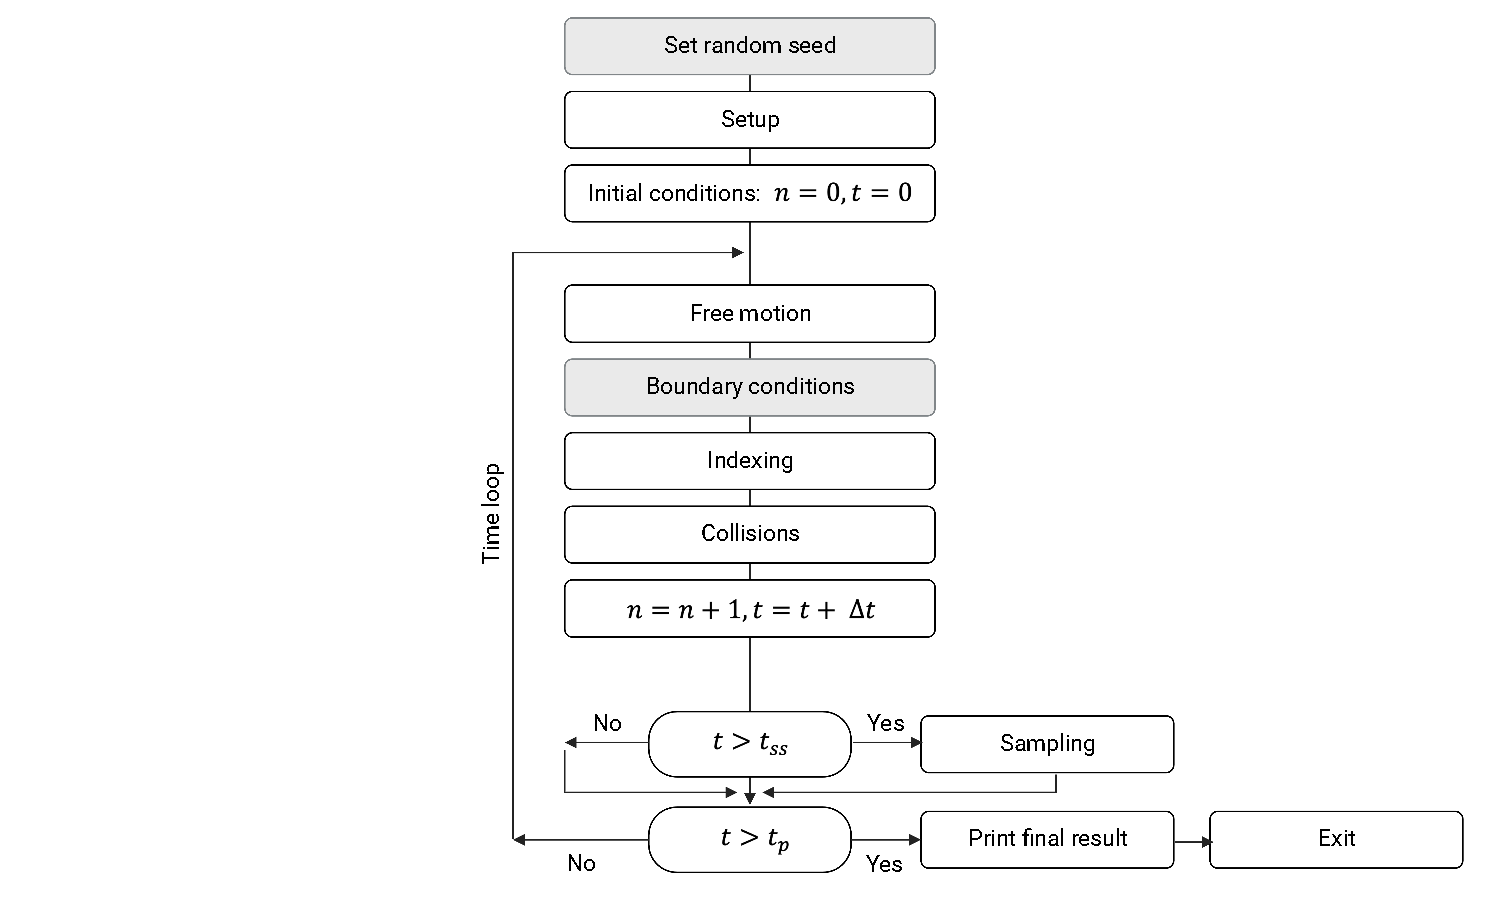
\includegraphics[width=\textwidth]{../Images/3. Methodology/dsmcflowchart.pdf}
    \caption{Flowchart of DSMC method loop. Adapted from \cite{dsmcnotes}.}
    \label{fig:dsmcflowchart}
\end{figure}